\chapter{Background}
Waves exhibit many characteristics when travelling through different media.
Much research has been carried out to investigate and harness these properties
to develop technologies and devices which manipulate electromagnetic and also
acoustic waves.

\section{History}
Since the earliest days of human history, we have sought to better understand
the natural world around us and so create technologies to improve our lives. At
first by utilising what nature already has to offer, but later on developing
materials and devices which have desirable properties not found in nature.

This progression describes roughly how the study of metamaterials came about.
It began in 1887 with the study of how certain crystals exhibit interesting
iridescence.\cite{pcearliest} After two independently developed landmark papers
were published in 1987 on structures with band gaps for electromagnetic
waves,\cite{pceli,pcjohn} the term photonic crystal --- a periodic optical
nanostructure which manipulates the passage of electromagnetic radiation ---
was coined.\cite{pcfocus} Since then, photonic crystals have been mass produced
and used for many purposes, e.g. optical fibres for transmission of digital
information \cite{pcopfib} and precision surgery.\cite{pcsurgery,pcneuro}

Then came the study of metamaterials --- materials engineered to possess some
property not found in naturally occurring materials.\cite{briefintro} Usually
these materials are composed of smaller units which are arranged in a repeating
pattern. They derive their properties not from the intrinsic properties of the
base materials, but from the periodic structure introduced.

One of the first major breakthroughs which the study of metamaterials led to
was the development of materials with a negative refractive index. Though the
possibility of creating such a material was theoretically predicted in
1967,\cite{negrefrac} it was only experimentally verified in
2001.\cite{negrefracex}

Nowadays, there is much research being done in the area of topological
metamaterials or topological photonic
crystals.\cite{topoedge,toposplit,topomet} This is where new properties of
metamaterials are produced by perturbing their structures utilising topological
and group theoretic concepts, usually by breaking symmetries which are present
in the original material. The reason there is considerable interest in applying
these abstract fields to the study of metamaterials is due to their ability to
transcend specific physical systems and be applied widely. An example is being
able to create metamaterials which split energy in multiple
directions.\cite{toposplit} 

\section{Practical applications}
\label{applications}
Metamaterials have the potential to solve many modern engineering problems.

\begin{itemize}
\item Developing a cloak of invisibility.\cite{emcloak}
      \begin{itemize}
      \item Obvious use cases in military.
      \item Protect things from electromagnetic radiation.
      \end{itemize}
\item Constructing antennae to focus energy into narrow beams.
      \cite{diremi,antennasol}
      \begin{itemize}
      \item Gather wave energy from deep in the oceans and concentrate them to
            be harvested.
      \item Channel sound energy, e.g. from train tracks, to be dissipated
            elsewhere which decreases noise pollution.
      \end{itemize}
\item Producing devices which operate on the terahertz ($1THz=10^{12}Hz$)
      range.\cite{THz}
      \begin{itemize}
      \item Can be used in medical imaging due to terahertz radiation being
            able to penetrate thin materials but not thicker objects. Also, it
            is non-ionising radiation and so does not damage living cells
            unlike X-rays.
      \item For surveillance, especially security screening as many materials
            of interest have unique spectral fingerprints in the THz
            range.\cite{Thzsec}
      \end{itemize}
\item Developing near perfect electromagnetic absorbers.\cite{absorbing}
\item Developing energy splitters.\cite{toposplit}
\item Developing perfect lenses.\cite{negrefraclens}
\end{itemize}

\section{Models studied}
There are many different models which we can use to study the effects of
metamaterials on the waves which propagate through them. 

\begin{figure}[!h]
\centering
\includegraphics[width=0.8\textwidth]{imgs/flexplate.png}
\caption{\label{fig:flexplate} Schematic view of a thin plate flexural wave
         model which consists of an array of resonators attached to a thin
         elastic plate. Each resonator is a point mass attached to the plate by
         a spring. Image adapted from source.\cite{graphene}}
\end{figure}

In the literature, thin plate flexural wave theories,\cite{graff,toelastic} as
seen in Figure~\ref{fig:flexplate}, have proven to be highly effective physical
models and reliable predictors of physical wave phenomena as shown by the
numerous studies done on flexural (or bending) waves in a beam or a
plate.\cite{flexbeam,graphene,mehulgeom} This is very advantageous as most
acoustic (or sound) radiation travels as flexural waves through structures and
deforms the medium transversely as they propagate.\cite{sound} Therefore, these
models are very useful in studying acoustic metamaterials or phononic
crystals.\cite{phonon} As a specific example, an elastic analogue of graphene,
a honeycomb arrangement of mass-spring resonators attached to a thin elastic
plate, was shown which could be used as waveguides.\cite{graphene}

Having said that, the equations which govern the propagation of flexural waves
are much more complicated than those for a simple mass-spring system and
requires more background knowledge in its physics to properly understand and
implement. As an example, the biharmonic equation which governs the propagation
of flexural waves in a lattice of mass-spring resonators is a fourth-order
partial differential equation.

Along the same lines, the modelling of electromagnetic metamaterials present
the challenges of getting to grips with the theory of electromagnetic
radiation, e.g. Maxwell's equations\cite{maxwell} and Bragg
scattering\cite{bragg}.

\begin{figure}
\centering
  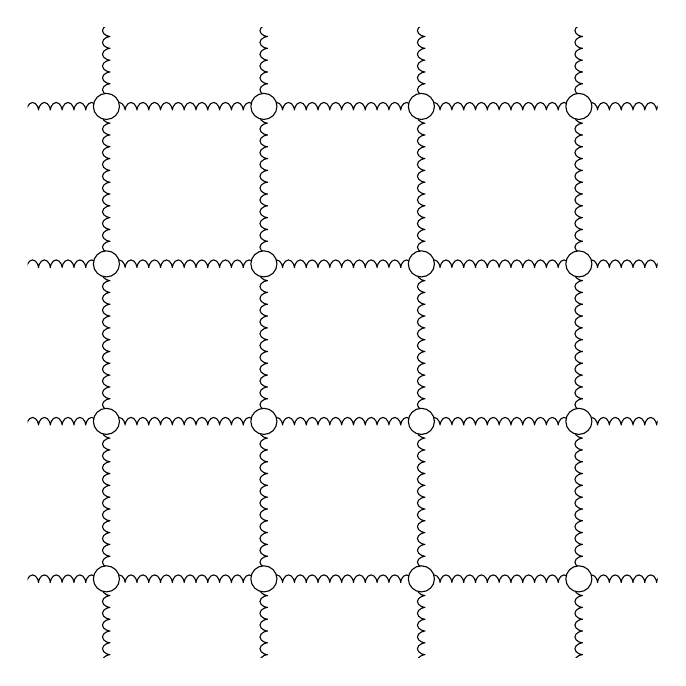
\begin{tikzpicture}
    \clip (-1,-1) rectangle (7,7);
    \foreach \X in {-2,0,...,6}
    {\foreach \Y in {-2,0,...,6}
     {\draw[decorate,decoration={coil,aspect=0.5,amplitude=0.5mm, segment
    length=1.5mm}] (\X,\Y) -- ++(0,2) -- ++(2,0);
    \node[circle,draw,inner color=white] at (\X,\Y) {};}}
  \end{tikzpicture}
  \caption{\label{fig:ourmodel} Schematic view of our simple mass-spring model.}
\end{figure}

Given the timeline of this project, the limited Physics background I have, as
well as to make the results accessible to a wider audience, we have decided to
go for a simplistic masses-connected-by-springs model, as seen in
Figure~\ref{fig:ourmodel}, as the core object of study in our project. Not only
does this reduce the complexity as we only need to deal with ordinary
differential equations and not partial differential equations, it also reduces
the complexity in the scattering simulations as we now have to solve a discrete
system instead of a continuous one. With this \textit{toy} system, we will be
able to more quickly lay the foundations required to carry out more interesting
experiments, from which results can be transferred to other models.

The following will be brief explanations of concepts which will form the
foundation on which we will analyse and investigate the properties of our
lattices.

%TODO: Write a litle background on the following
\section{Bloch waves}

\section{Dispersion relation}

\section{Brillouin zone}

